% =============================================================================================
% 2 Methods. Each paragraph <= 100 words (user constraint).
% v2 (2026-10-24 evening): EDA rewritten as findings -> design; timeline figure moved here; M0 figure added;
% contralateral-information statement added to the pipeline paragraph.
% =============================================================================================
\section{Methods}
\label{sec:methods}

\paragraph{Overall design.}
The unit of analysis is the hip; resampling is by participant. The outcome is ipsilateral THA within ten years. It is
defined by the prosthesis flag, the first post-operative visit, or a prosthesis recorded on a follow-up film. The reading
file stores the last case as code 5 in the KL field. This is not a KL grade (KL ends at 4); it never occurs at baseline,
and 89 of the 91 hips with this code are replaced hips. Every disagreement was checked against the films. Clinical tables feed M0 (elastic net), M1 (LightGBM), M1b (EBM) and M2 (FT-Transformer). The
radiograph feeds M3, a supervised image head, and the fusion model gives M0 the cross-fitted M3 logit
(Fig.~\ref{fig:overview}). Estimates come from 5$\times$5 nested cross-validation (CV), with AUPRC as the primary metric.
Figure~\ref{fig:timeline} places every input and label on the study timeline.

\begin{figure}[!tbp]
  \centering
  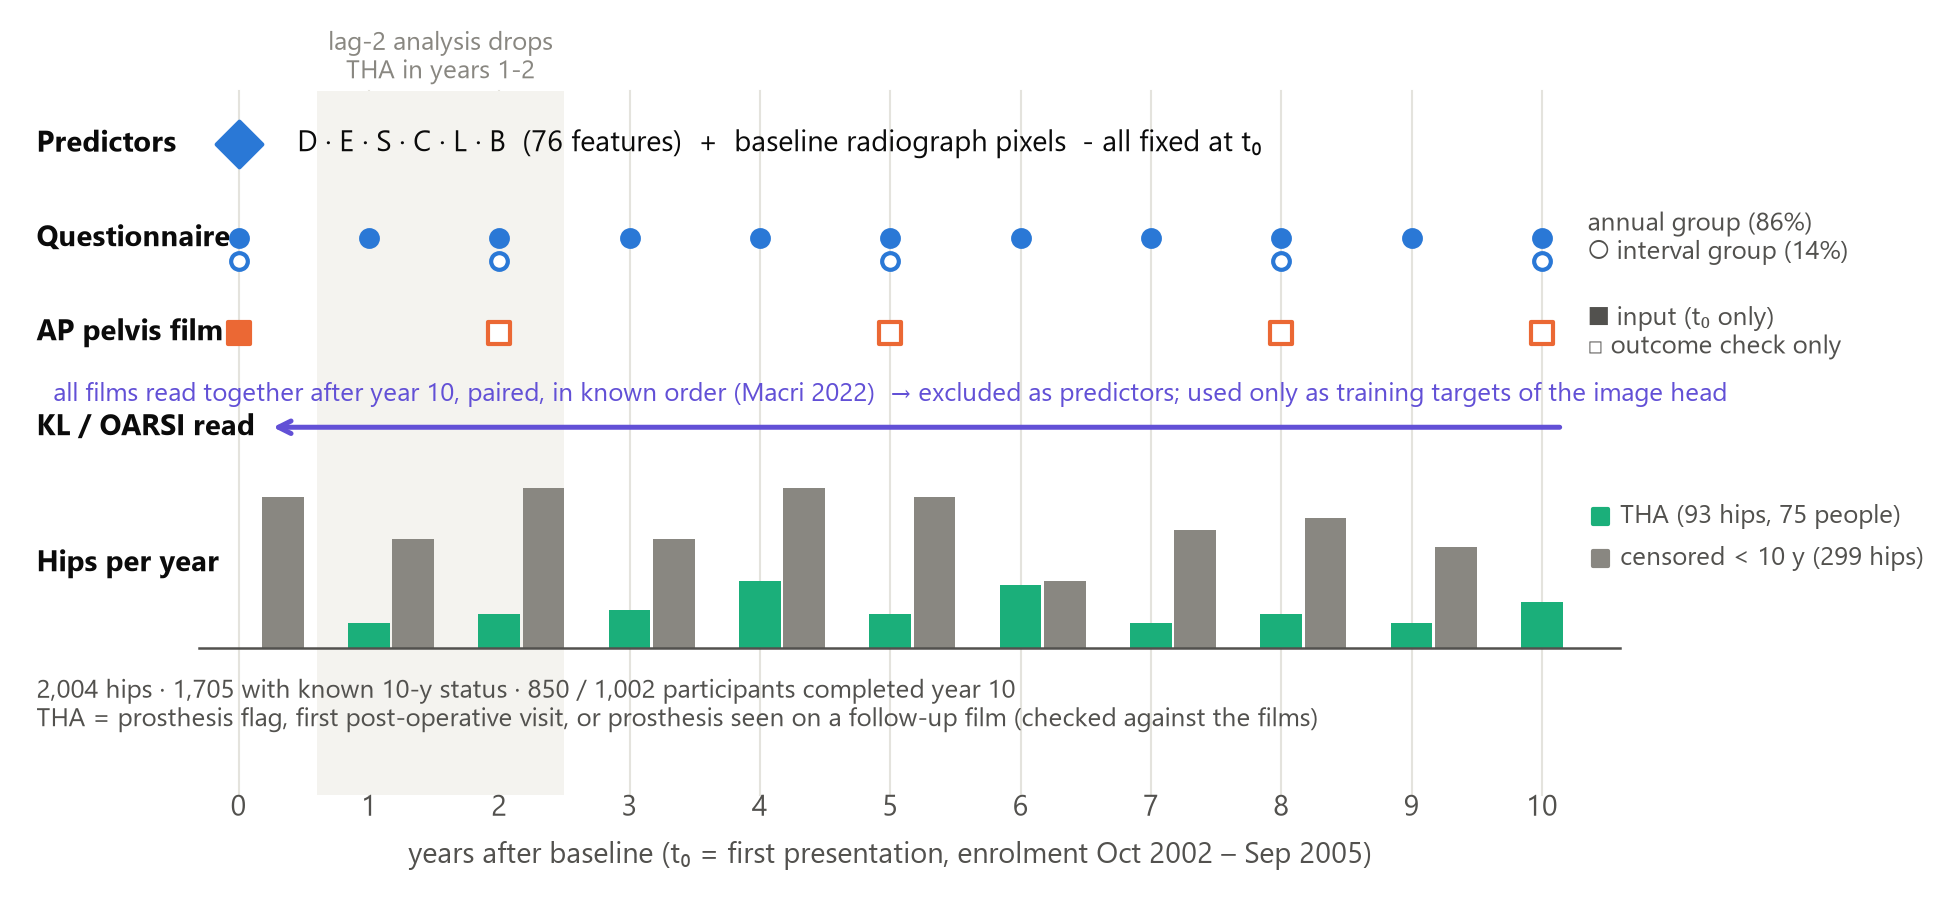
\includegraphics[width=\linewidth]{fig2_timeline.png}
  \caption{\textbf{Study timeline and the admissibility of each input.} Predictors are restricted to values fixed at
  $t_0$: the six clinical feature groups and the baseline AP pelvic film. Later questionnaires and films serve only to
  define THA and censoring. The public KL/OARSI readings were scored after year 10 with all films side by
  side~\cite{macri2022}; they are therefore excluded as predictors and used only as training targets of the image head.
  Bars show THA (green) and censoring before year 10 (grey) per year; 152 of 1,002 participants did not complete year 10
  (older, more often not in paid work; standardised mean differences $\le0.18$). The shaded band marks the events
  removed in the lag-2 analysis.}
  \label{fig:timeline}
\end{figure}

\paragraph{Exploratory analysis: cohort and outcome.}
No exploratory step used model fits. Of 2,004 hips, 1,705 have known 10-year status and 93 were replaced
(Fig.~\ref{fig:s-flow}); the Kaplan--Meier 10-year risk is 5.1\%. Risk differed sharply by ipsilateral hip pain (10.2\%
vs 1.7\%) and by internal rotation $\le25^\circ$ (10.5\% vs 2.7\%), but little by visiting group or film format
(Fig.~\ref{fig:s-km}). Across the ten recovered centres it ranged from 1.7\% to 7.9\% (Fig.~\ref{fig:s-km-centre};
participant-clustered GEE $p=0.36$). The two hips of a participant are dependent: a quarter of participants with one
THA also had the other hip replaced.

\paragraph{Exploratory analysis: examination and symptoms.}
Examination items were graded rather than threshold-like. Per standard deviation, internal-rotation ROM had univariable
OR 0.46 and flexion ROM 0.54; each grade of pain on internal rotation or flexion had OR 2.0 and 1.7. Contralateral
internal rotation still carried signal (OR 0.76). Dichotomising internal rotation at $25^\circ$ (OR 4.1) discards this
gradient. Ipsilateral hip pain was the strongest symptom (OR 6.0), WOMAC function and pain were weaker (1.4/SD), and
biomarkers were weak ($\le1.34$/SD). Ipsilateral knee pain had OR 0.43. This pattern marks ``bystander'' hips, which
were enrolled because of the knee.

\paragraph{Exploratory analysis: collinearity, missingness and distributions.}
Several inputs measure the same construct twice. Left and right ROM correlate at $\rho$ = 0.77--0.84, each ROM correlates
with its own cut-off ($\rho\approx-0.8$), current and weekly pain correlate at 0.83, and the WOMAC total is the exact sum
of its subscales. Within the examination block, VIF reached 6.1. Missingness followed three mechanisms
(Fig.~\ref{fig:s-missing}). Some items were gated by a complaint or status (38 raw variables). Some depended on the
centre protocol (41), with missing rates of 0 or 1 by centre. The rest were sporadic (2--5\%; 92). Fifteen continuous
variables had $|\text{skew}|>1$ (Fig.~\ref{fig:s-skew}).

\paragraph{How the exploratory analysis shaped the design.}
Three principles followed. First, the model should not depend on which member of a correlated pair it picks. M0
therefore uses an elastic-net penalty, whose $\ell_2$ part spreads weight across correlated features; inner tuning chose
ridge-dominant mixing ($\ell_1$ ratio 0.1--0.3) in 20 of 25 outer folds. Trees and the FT-Transformer handle correlation
natively. Second, when two inputs carry the same information, the one closer to clinical practice and easier to obtain
enters the model; the other is kept for reference. Third, no input may encode the centre through its missingness.

\paragraph{}
The second principle kept the continuous ROM and pain grades, with the $25^\circ$/$115^\circ$ cut-offs used only for
description. It kept the weekly pain score, which depends less on the visit day, and the WOMAC subscales rather than
their sum. Contralateral values enter as asymmetry terms (ipsilateral minus contralateral). Under the third principle,
external rotation, adduction and abduction ROM and the bursitis/tendinitis tests left the main set because of their
centre-specific missingness, not their signal; they enter sensitivity analyses only. The final set has 76 features,
maximum VIF 5.1, and three pairs with $|\rho|\ge0.7$ (Fig.~\ref{fig:corr}).

\begin{figure}[!tbp]
  \centering
  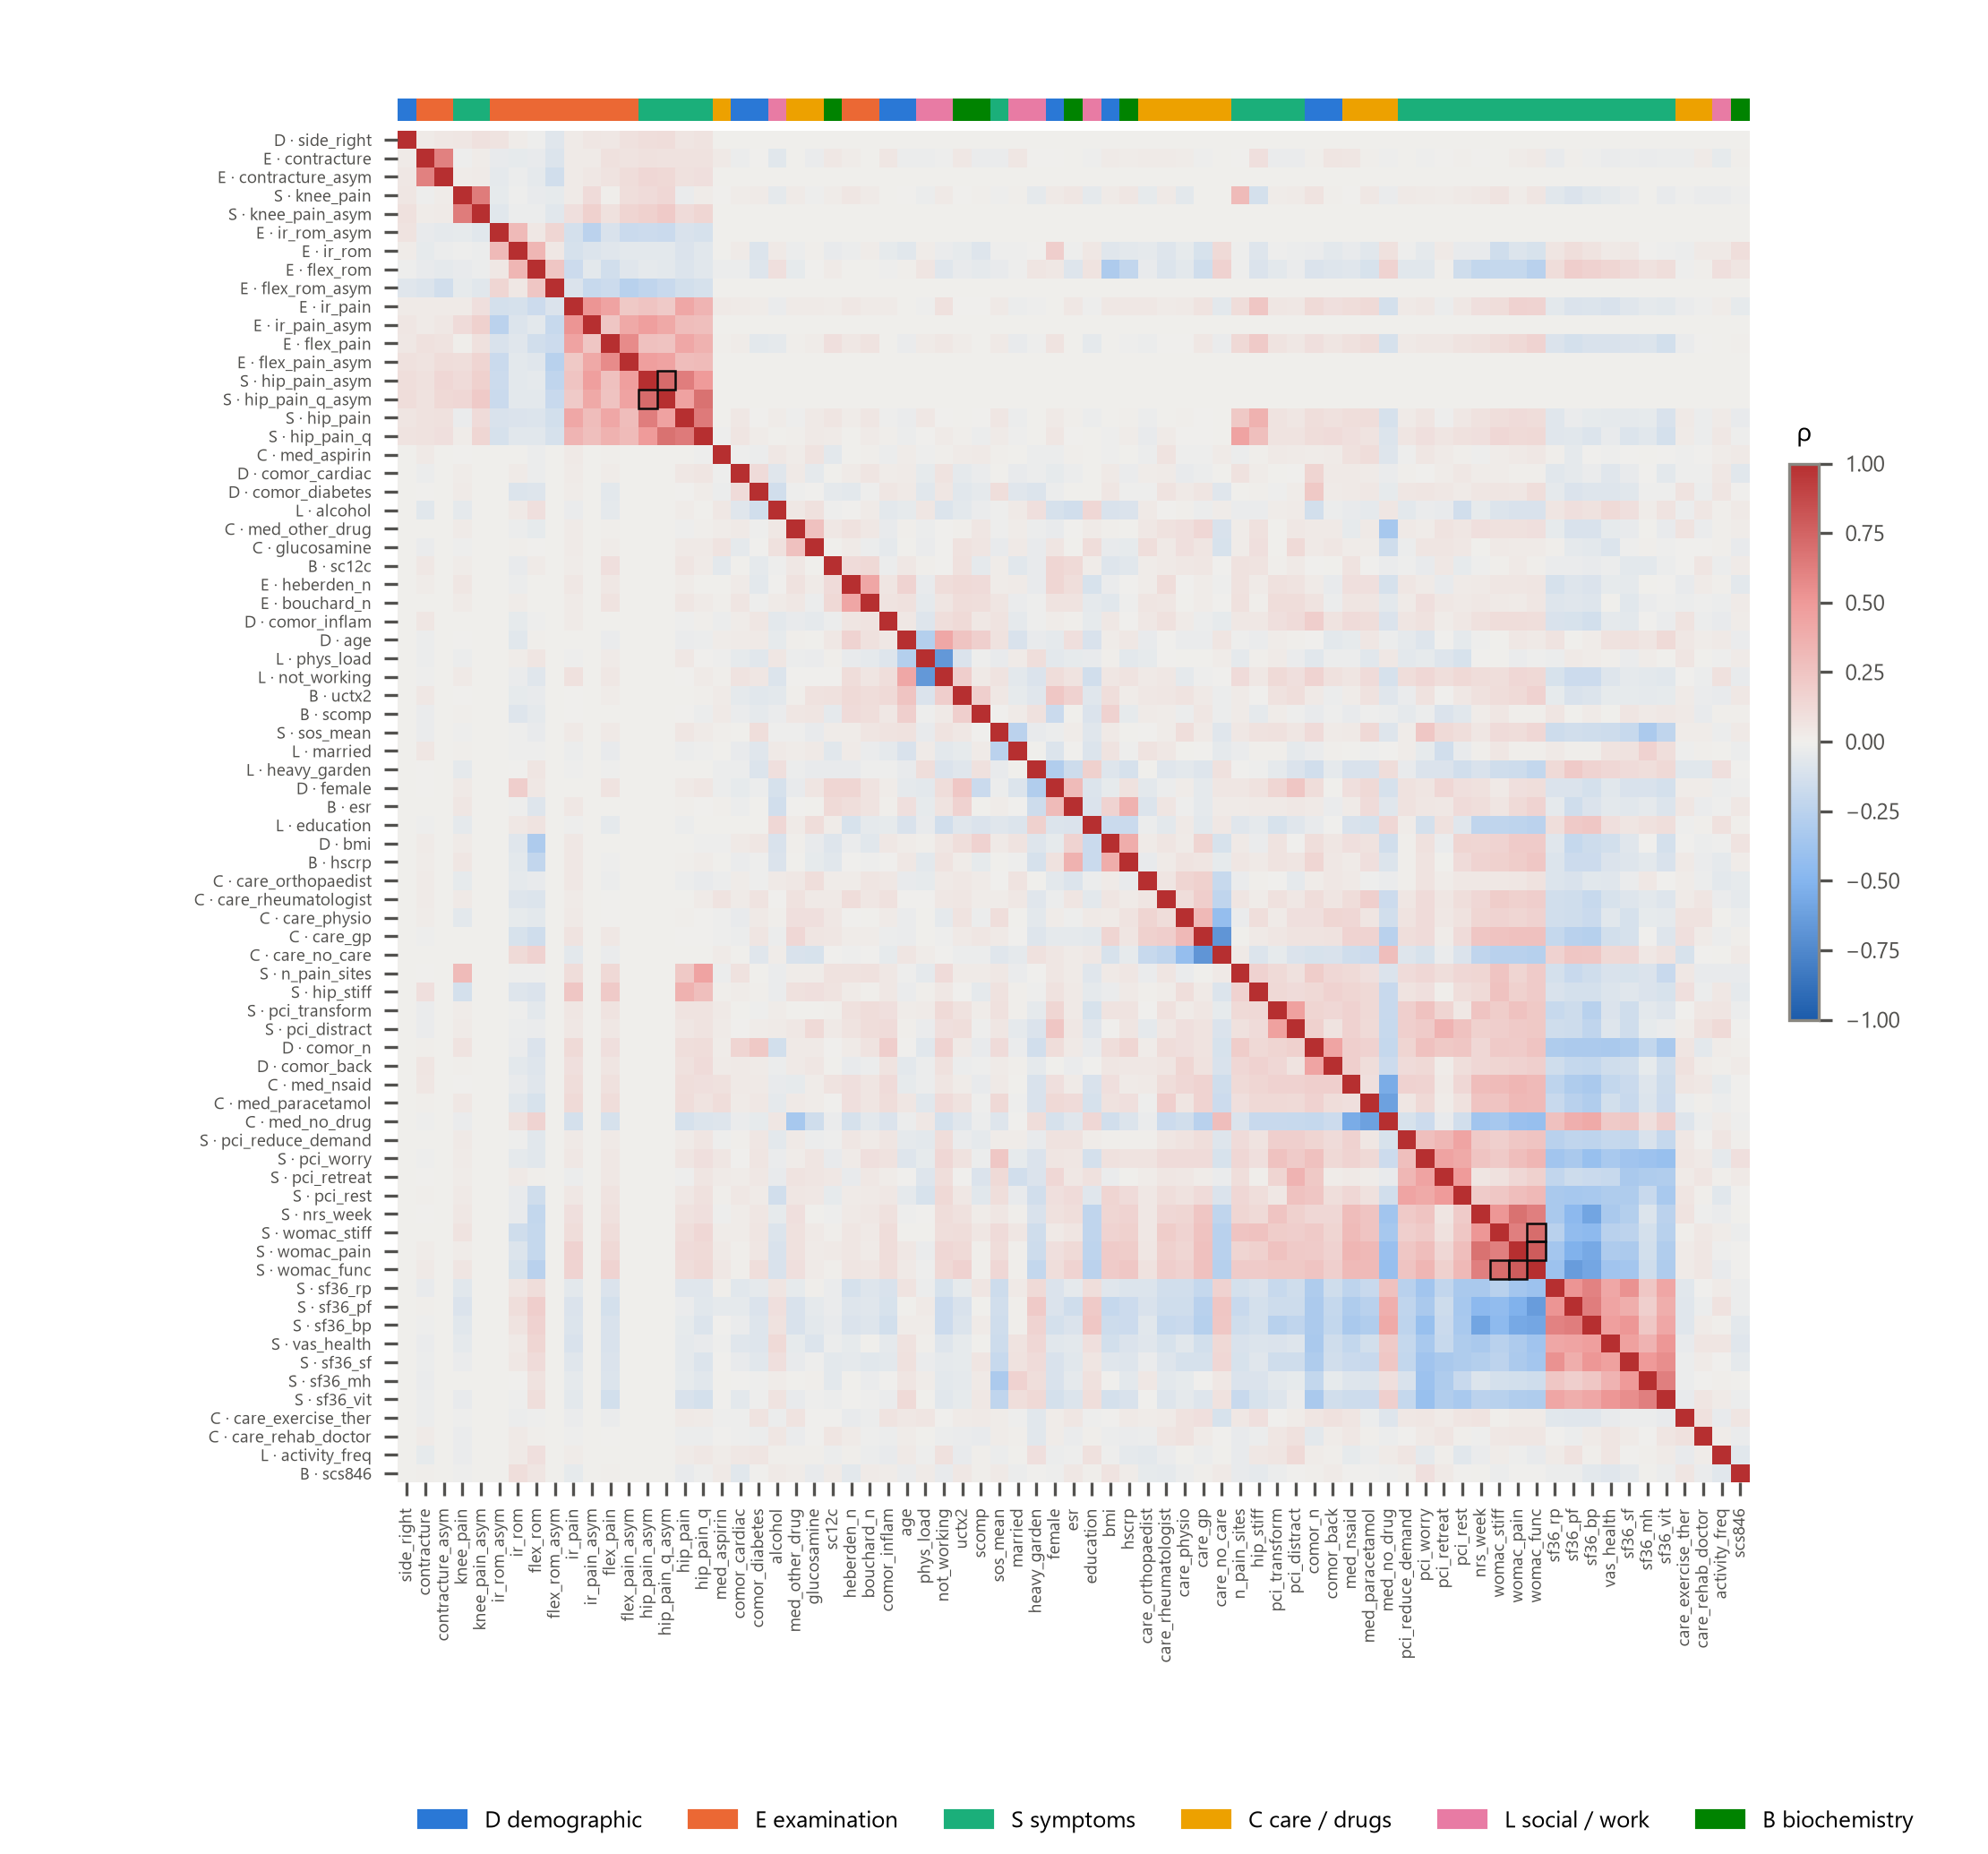
\includegraphics[width=0.92\linewidth]{fig3_correlation.png}
  \caption{\textbf{Spearman correlation of the 73 numeric main features} (three nominal features not shown), ordered
  by hierarchical clustering; the strip marks the feature group. Boxed cells: $|\rho|\ge0.7$, namely WOMAC
  pain--function (0.79), WOMAC stiffness--function (0.71) and the two hip-pain asymmetry terms (0.71). The symptom
  scales form one block. Hip-examination items cluster with ipsilateral hip pain, and SF-36 domains form an inverse block.}
  \label{fig:corr}
\end{figure}

\paragraph{Data partition and pipeline.}
Folds are stored once and shared by every model (Fig.~\ref{fig:pipeline}). The outer loop is 5-fold
StratifiedGroupKFold, repeated five times. It is grouped by participant and stratified by the participant's number of THAs
(0/1/2) $\times$ film format, which gives 17--20 events per test fold. Inside each outer training set, three
participant-grouped inner folds serve hyper-parameter selection, early stopping, Platt calibration and cross-fitting of
the image logit. We report the mean over repeats of each pooled out-of-fold metric. 95\% CIs (500 draws) and paired
differences ($\Delta$; 1,000 draws) come from a participant-clustered bootstrap of repeat~0.

\paragraph{No information from the other hip beyond baseline.}
A model scoring one hip sees the other hip only through $t_0$ values. Asymmetry terms are computed from the baseline
table. The image crop contains one hip, and the auxiliary reading targets are ipsilateral. The other hip's follow-up
data, including its THA, are never inputs. Both hips of a participant always fall in the same fold, so the other hip's
label cannot cross a train/test boundary. The participant's THA count is used only to stratify the folds. We verified
each of these points in the code.

\begin{figure}[!tbp]
  \centering
  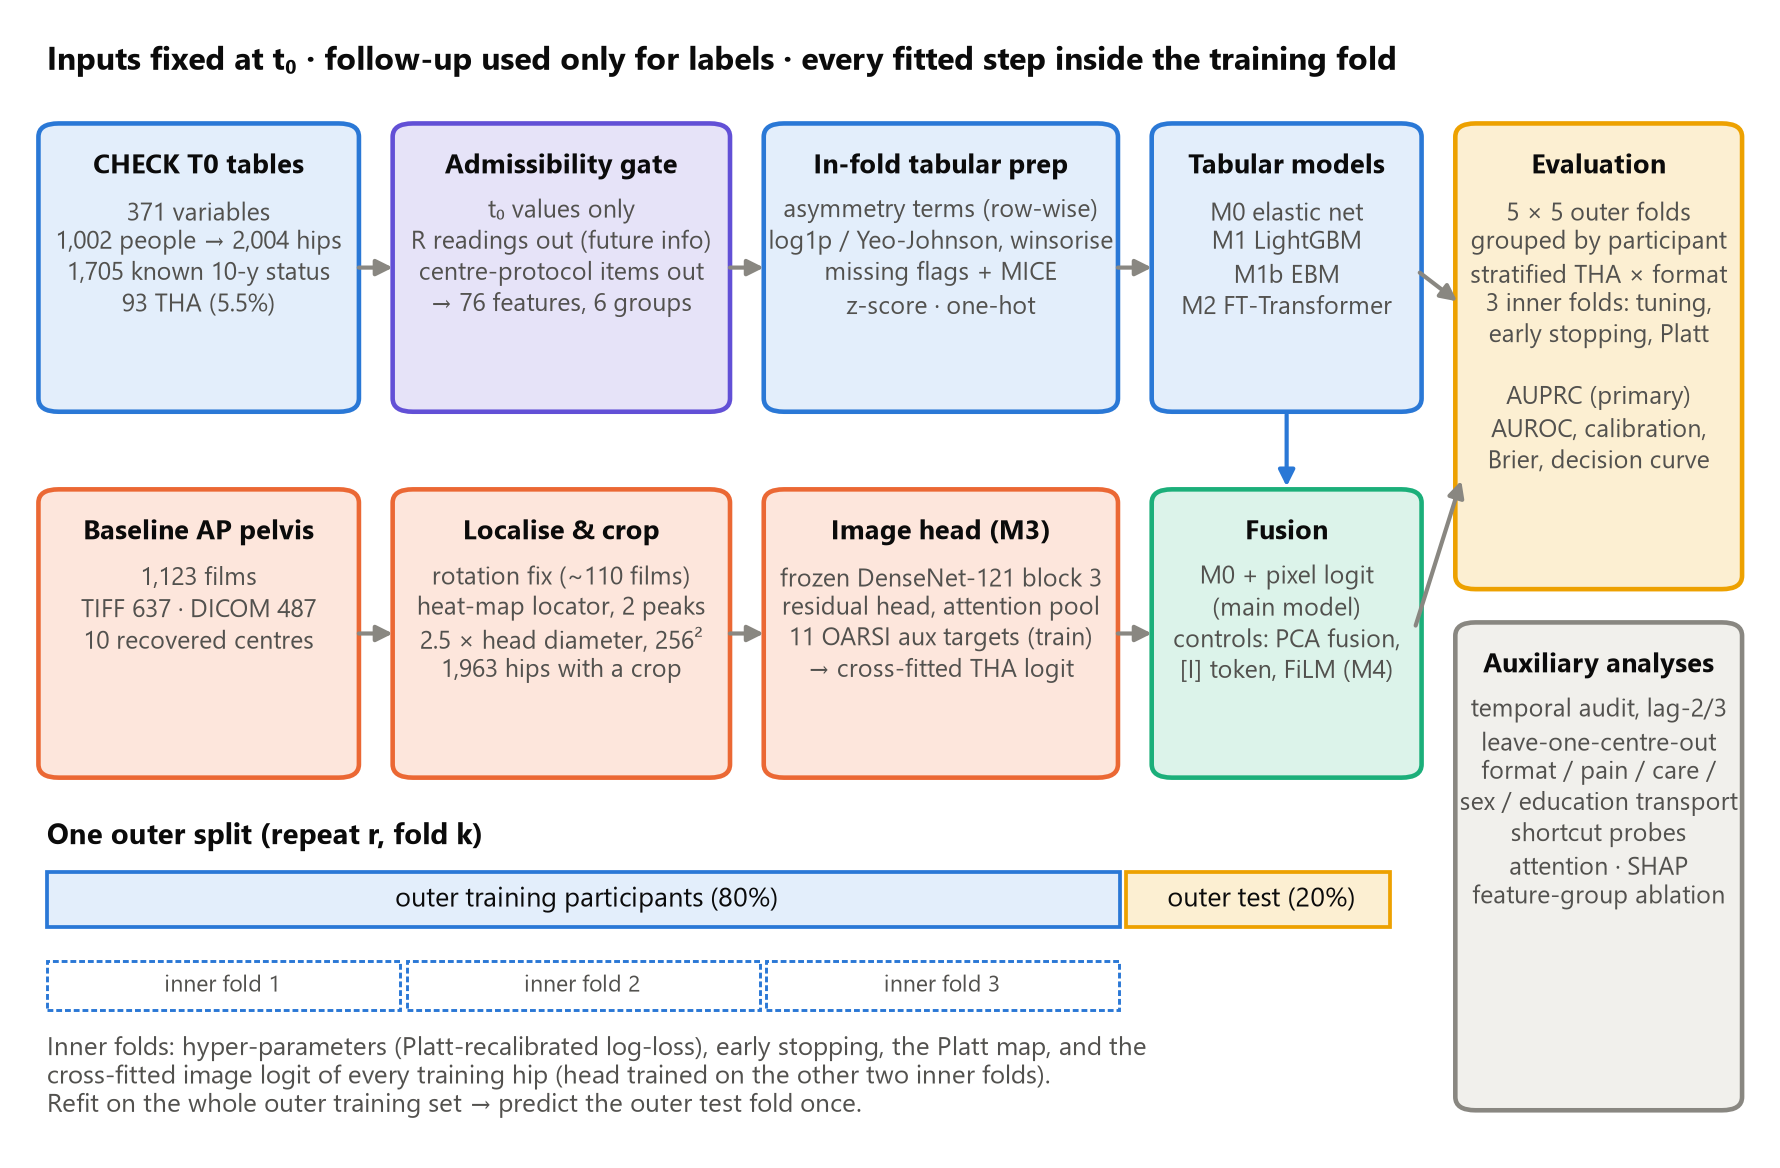
\includegraphics[width=\linewidth]{fig4_pipeline.png}
  \caption{\textbf{Pipeline and fold layout.} Inputs pass an admissibility gate (values fixed at $t_0$ only). Tabular
  preprocessing is fitted inside each training fold. The image path is reorientation, femoral-head localisation,
  cropping, frozen DenseNet features and the trainable head, whose logit is cross-fitted. Bottom: one outer split; the
  three inner folds are used for tuning, early stopping, Platt calibration and cross-fitting.}
  \label{fig:pipeline}
\end{figure}

\paragraph{Preprocessing without leakage.}
A line-by-line code audit confirmed that every fitted step runs on the current training rows only, in this order:
\begin{enumerate}[leftmargin=*,itemsep=0pt,topsep=2pt]
  \item row-wise asymmetry terms and structural rules (below);
  \item log1p for biomarkers and Yeo--Johnson for other variables with $|\text{skew}|>1$, both fitted on training rows
        (Fig.~\ref{fig:s-skew});
  \item winsorising at the training 0.5/99.5\% quantiles;
  \item missing indicators;
  \item MICE imputation of sporadic gaps (BayesianRidge, 10 rounds, outcome excluded);
  \item $z$-scoring and one-hot coding.
\end{enumerate}
Validation and test rows are only transformed. Trees keep NaN, and the FT-Transformer uses a learned per-feature [MISS]
token. Three label-free steps used all rows: the transform type per variable, the redundancy rules, and the
image-normalisation models below.

\paragraph{Structural rules.}
Gated items are not missing at random, so they were coded from the questionnaire logic (Fig.~\ref{fig:s-missing}). Hip
morning stiffness was asked only of participants who reported hip complaints: it is missing in 9\% of hips without hip
pain and in none with pain. A skipped item therefore means ``no hip complaint reported'' and is coded as no stiffness.
Physical workload was asked only of people in paid work, so non-workers receive the lowest level plus a not-working
indicator. Menopause has its own category for men. Missing categories get an indicator.

\paragraph{Image preprocessing and annotation.}
There were 1,123 baseline films (637 digitised-film TIFF scans, 487 DICOM). About 110 TIFF scans were stored rotated by
$90^\circ$. A self-supervised four-way rotation classifier (ResNet-18; 98.5\% accuracy on held-out rotations) restored
them. We annotated femoral-head centres and radii on 162 stratified films (279 heads) and trained a ResNet-18 U-net
heat-map locator on them. Decoding two peaks gave a median error of 0.27 head radii (3-fold subject CV). Crops measure
$2.5\times$ head diameter at $256^2$, 16 bit, with left hips mirrored. After visual QC, 1,963 hips have a crop,
including every THA hip.

\paragraph{Tabular models.}
M0, the reference and the clinical part of the final model, is an $\ell_1/\ell_2$-penalised logistic
regression~\cite{zou2005elasticnet} on the preprocessed features (Fig.~\ref{fig:m0}). Its 40 candidate configurations
span $C$ from $1.5\cdot10^{-3}$ to 9.6 (log scale), $\ell_1$ ratio from 0 to 1 and class weighting on or off. M1 is
LightGBM with depth-limited trees and class weights~\cite{ke2017lightgbm}. M1b is an explainable boosting
machine~\cite{nori2019interpretml}, the same model family as Jang's GAM~\cite{jang2023}.

\paragraph{}
We did not resample the data (no SMOTE), because imbalance correction does not improve discrimination and harms
calibration~\cite{vandengoorbergh2022}. We used class weights or focal loss instead, followed by Platt
recalibration~\cite{platt1999} fitted on inner out-of-fold predictions. All candidate configurations were drawn once
with a fixed seed, and every outer fold scores the same list.

\begin{figure}[!tbp]
  \centering
  \IfFileExists{figs/fig5_m0.png}{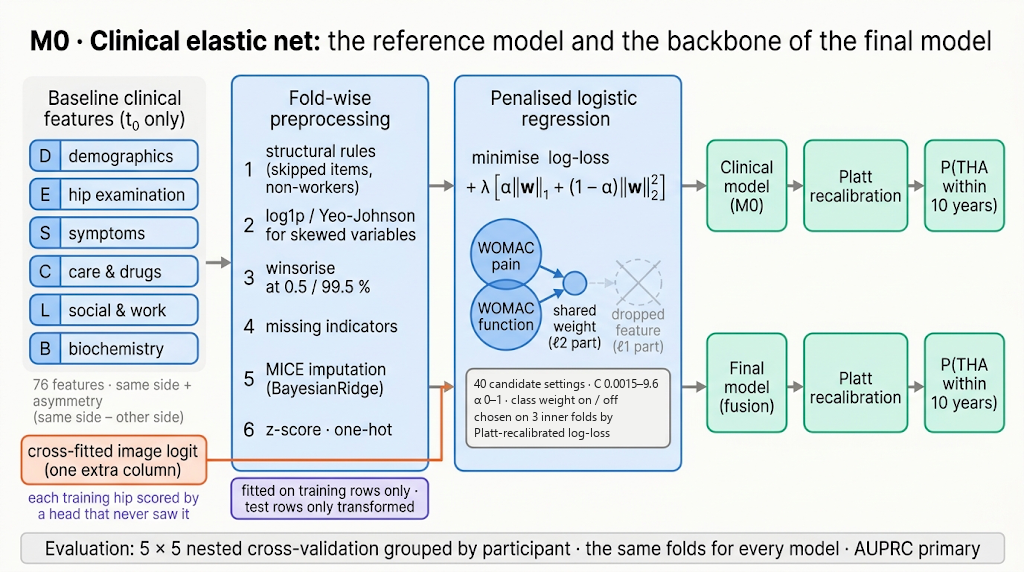
\includegraphics[width=\linewidth]{fig5_m0.png}}{%
    \fbox{\parbox[c][4cm][c]{0.95\linewidth}{\centering\todo{fig5\_m0.png: M0 diagram (Gemini prompt in figure\_prompts\_gemini.md)}}}}
  \caption{\textbf{M0 clinical elastic net and its use in the final model.} Raw baseline features pass the fold-wise
  preprocessing chain (asymmetry and structural rules, skew transforms, winsorising, MICE with missing indicators,
  $z$-scoring and one-hot coding). An $\ell_1/\ell_2$-penalised logistic regression, tuned on three inner folds by
  Platt-recalibrated log-loss, gives the clinical model. In the final model the same learner receives one extra column,
  the cross-fitted image logit, and its output is Platt-recalibrated.}
  \label{fig:m0}
\end{figure}

\paragraph{Feature engineering for the FT-Transformer.}
The FT-Transformer receives the same $z$-scored numerics (Fig.~\ref{fig:ftt}). Each feature $j$ becomes a $d$-dimensional
token,
\[
  t_j = \phi_j(x_j) + e_j + g_{\mathrm{group}(j)},
\]
where $\phi_j$ is a linear, periodic or piecewise-linear value embedding (bins from training quantiles), $e_j$ a learned
feature-ID embedding and $g$ a group embedding. Categorical features use embedding tables. A [CLS] token is prepended.
All three tokeniser types entered the architecture search; the selected architectures use the linear one.

\begin{figure}[!tbp]
  \centering
  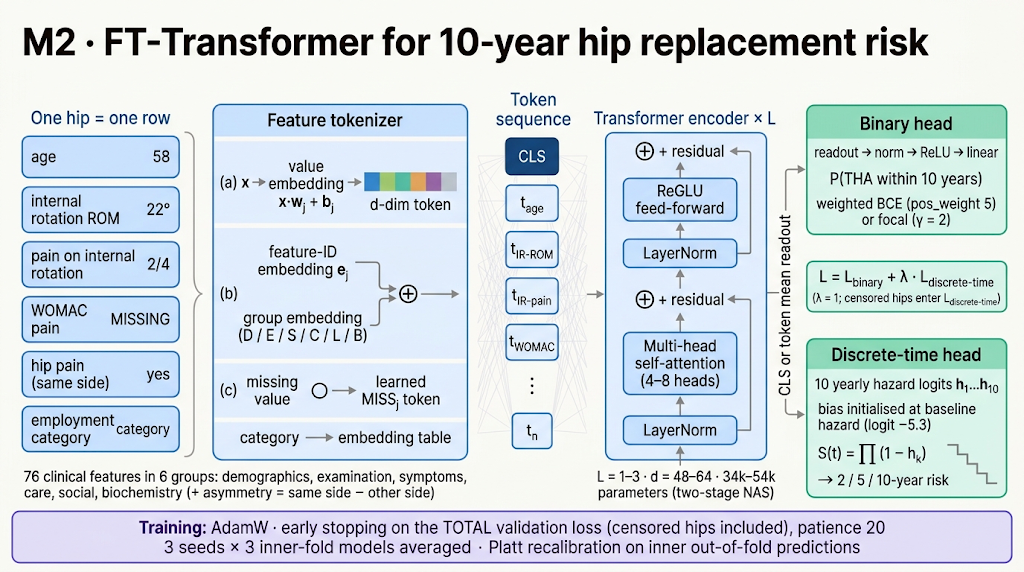
\includegraphics[width=\linewidth]{fig6_ftt.png}
  \caption{\textbf{M2 FT-Transformer.} Each hip is one row; every feature becomes a token (value embedding + feature-ID
  + group embedding; a learned [MISS]$_j$ token replaces missing values). Pre-norm Transformer blocks with residual
  connections feed a binary head and a discrete-time head with ten yearly hazards. The two are trained jointly
  ($\lambda=1$), and censored hips contribute through the discrete-time term.}
  \label{fig:ftt}
\end{figure}

\paragraph{M2: FT-Transformer and its stabilisation.}
M2~\cite{gorishniy2021fttransformer} stacks $L$ pre-norm blocks (multi-head self-attention, then a ReGLU feed-forward
layer), each wrapped in a residual connection. The loss is $\mathcal L=\mathcal L_{\text{bin}}+\lambda\mathcal
L_{\text{DT}}$. Here $\mathcal L_{\text{bin}}$ is weighted BCE (pos\_weight 5) or focal loss on hips with known status,
and $\mathcal L_{\text{DT}}$ is the discrete-time likelihood over all hips at risk. The first version had two faults. The
hazard bias started at 0, so the discrete-time head never trained, and early stopping on about 25 noisy validation
events made repeats unstable. The final recipe initialises the bias at the baseline hazard logit ($-5.3$), stops on the
total loss including censored hips, and averages three seeds. LayerNorm was compared with BatchNorm.

\paragraph{M3: image head.}
M3 uses an ImageNet DenseNet-121~\cite{huang2017densenet}, frozen, up to dense block 3. This yields a
$1024\times14\times14$ map in which one cell spans about a third of a head radius. The trainable head
(Fig.~\ref{fig:image-branch}; about 0.21\,M parameters) has four parts:
\begin{enumerate}[leftmargin=*,itemsep=0pt,topsep=2pt]
  \item a $1\times1$ convolution to 64 channels with BatchNorm;
  \item two residual blocks~\cite{he2016resnet};
  \item attention pooling~\cite{ilse2018attention} concatenated with global average pooling;
  \item one THA logit plus 11 auxiliary regressions onto the standardised OARSI items~\cite{altman2007oarsi}.
\end{enumerate}
The loss is $\mathrm{BCE}_{w=5}+\frac{1}{\sum_k m_k}\sum_k m_k(\hat r_k-\tilde r_k)^2$ over the available items $m_k$.
Readings are targets only, never inputs.

\paragraph{Training and cross-fitting of the image logit.}
The head trains for 30 fixed epochs (AdamW, 3-epoch warm-up, cosine decay, $\pm1$-cell shifts, Dropout2d 0.1). An inner
fold holds only about 25 events, too few for early stopping. Auxiliary targets are standardised within the training
fold. Within each outer training set the head is trained three times, each time without one inner fold, and scores the
hips of the fold it did not see. These out-of-fold logits are the image feature of the training hips. Test hips are
scored by a fourth head trained on the whole outer training set. M0 then refits with the logit as one extra feature
(stacking~\cite{wolpert1992stacked}).

\paragraph{}
Comparators were frozen PCA, a linear head, no auxiliary targets, AdaBN, SimCLR features, and [I]-token or FiLM fusion
of the frozen embedding into M2 (M4). Two follow-up runs were added. One fed the cross-fitted pixel logit as the [I]
token, with the same folds, architectures and single-seed recipe as the matching M2 run. The other (repeat 0)
restricted attention and average pooling to a disc of 1.6 head radii around the crop centre.

\begin{figure}[!tbp]
  \centering
  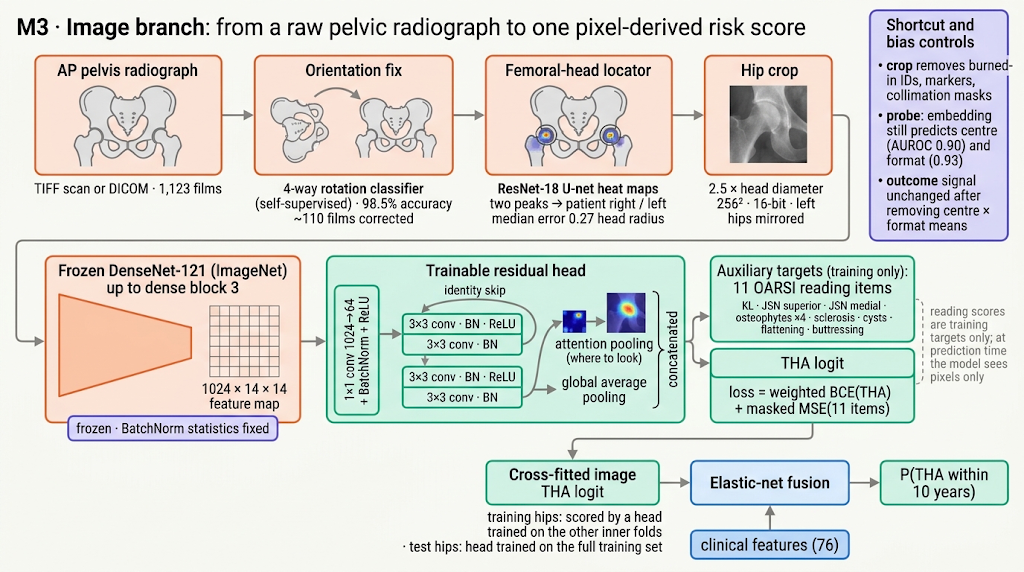
\includegraphics[width=\linewidth]{fig7_image_branch.png}
  \caption{\textbf{M3 image branch.} Raw film $\to$ orientation fix $\to$ femoral-head locator $\to$ hip crop $\to$
  frozen DenseNet-121 (block 3) $\to$ trainable residual head with attention pooling, supervised by the THA label and 11
  OARSI items (training only). The cross-fitted THA logit is the single image feature passed to the clinical elastic net.}
  \label{fig:image-branch}
\end{figure}

\paragraph{Hyper-parameter search and architecture search.}
Non-neural models were tuned by random search (40 configurations for M0, 60 for M1, 4 for M1b). Each outer fold selects
by Platt-recalibrated pooled inner log-loss, because inner AUPRC is unstable with about 25 events. M2 used a two-stage
search. Stage 1 scored 48 pre-sampled architectures (3.7k--56k parameters) on the inner folds of one outer split and kept
the best three. Stage 2 crossed them with lr $\{3\cdot10^{-4},10^{-3}\}$ and weight decay $\{10^{-5},10^{-4}\}$ inside
all 25 outer folds (Fig.~\ref{fig:hpo}; Table~\ref{tab:hparams}). The image head was not tuned.

\begin{figure}[!tbp]
  \centering
  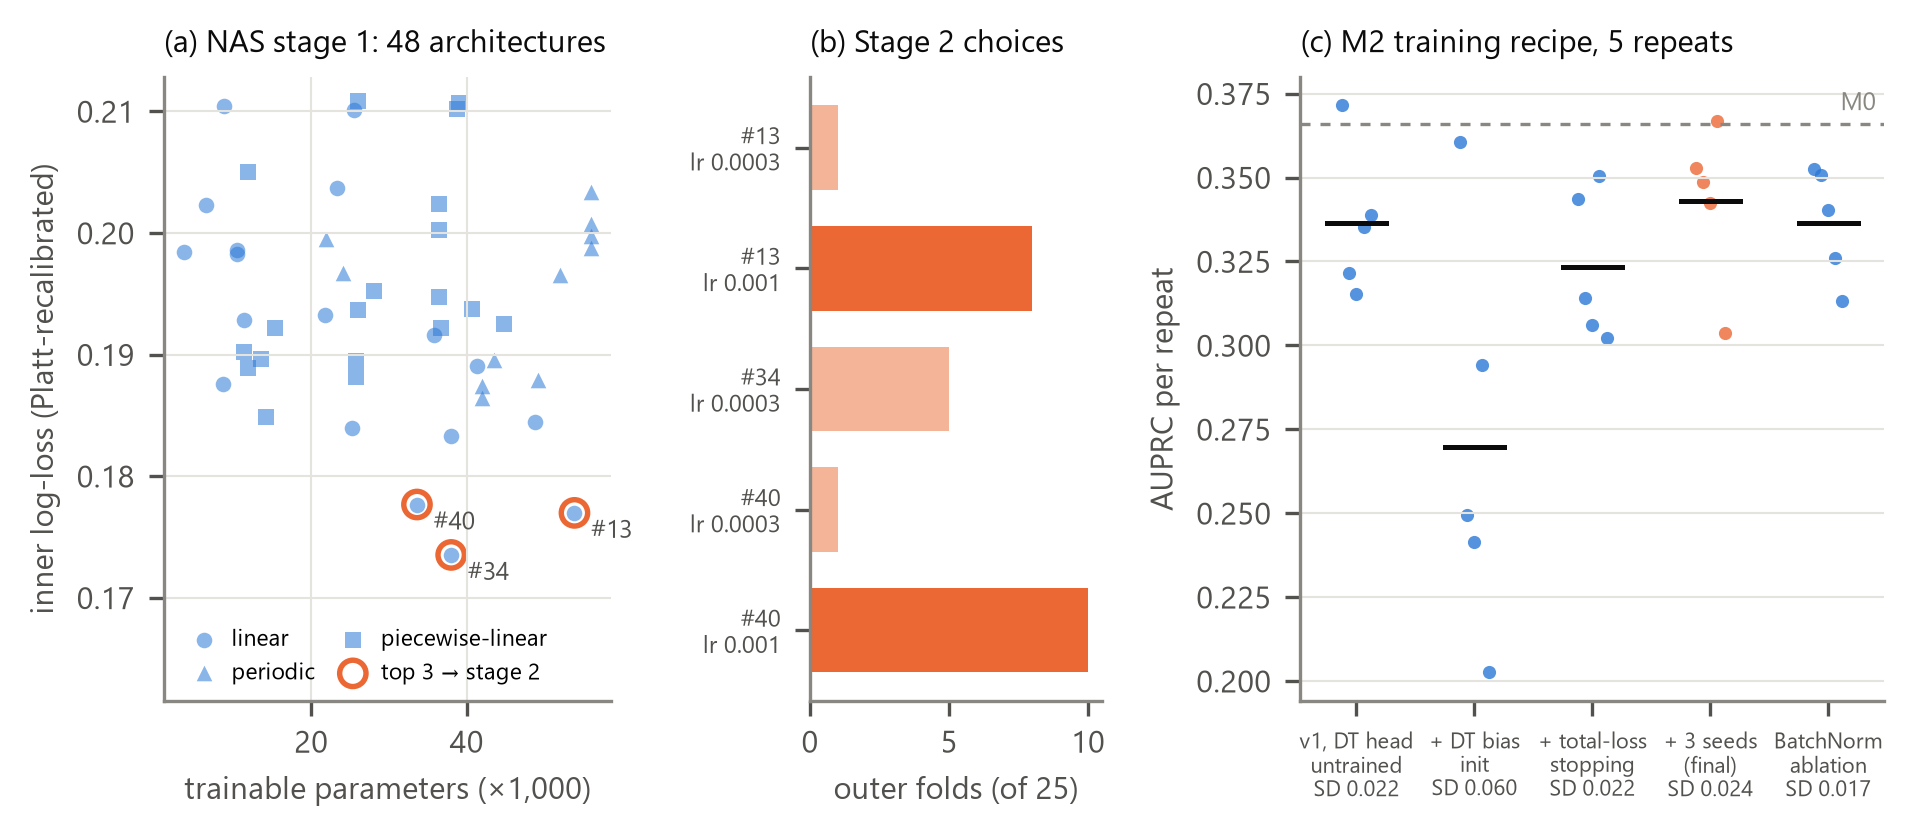
\includegraphics[width=\linewidth]{fig8_hpo_nas.png}
  \caption{\textbf{Hyper-parameter and architecture search.} (a) Stage-1 NAS: 48 FT-Transformer architectures, inner
  log-loss against size; the three best (circled) go to stage 2. (b) Configurations chosen across the 25 outer folds.
  (c) AUPRC of each repeat for successive M2 training recipes (bar = mean). The bias initialisation alone made the model
  unstable (SD 0.060), and early stopping on the total loss plus seed averaging restored stability (SD 0.024). The
  dashed line is M0.}
  \label{fig:hpo}
\end{figure}

% Table 2: final hyper-parameters. Sources: hpo/*.csv, oof/*_selection.csv, nas_stage1_DESCLB.csv, 08_imghead.py, lib_ftt.py
\begin{table}[!tbp]
  \centering
  \caption{\textbf{Search spaces and selected hyper-parameters.} ``Selected'' gives the configuration chosen most often
  across the 25 outer folds (count in brackets). M2's stage-2 choice varies by fold, so all three architectures are
  listed. The image head used fixed settings, chosen before training and not tuned per fold.}
  \label{tab:hparams}
  \small
  \setlength{\tabcolsep}{4pt}
  \begin{tabular}{@{}p{0.13\linewidth}p{0.40\linewidth}p{0.42\linewidth}@{}}
    \toprule
    Model & Search space & Selected / fixed \\
    \midrule
    M0 elastic net & 40 configs: $C\in[1.5\cdot10^{-3},9.6]$ (log), $\ell_1$ ratio $\{0,.1,.3,.5,.7,.9,1\}$, class
      weight \{none, balanced\}; SAGA & $C=0.012$, $\ell_1$ ratio 0.1, unweighted (10/25); next $C=0.082$, $\ell_1$ 0.3
      (6/25). The fusion model reuses this grid \\
    M1 LightGBM & 60 configs: leaves 4--31, depth 2--6, lr 0.01--0.10, min child 10--80, $\lambda_2$ 0.015--30,
      scale\_pos\_weight 1--20; early stop 100 rounds & leaves 31, depth 2, lr 0.042, min child 80, subsample 0.89,
      colsample 0.84, $\lambda_2$ 13.3, $\lambda_1$ 2.4, unweighted (5/25); median 232 trees \\
    M1b EBM & interactions \{0, 5\} $\times$ lr \{0.005, 0.02\}; 64 bins, min leaf 10, 8 outer bags & no interactions,
      lr 0.005 (16/25) \\
    M2 FT-Transformer & stage 1: 48 of $d\in\{16..64\}$, $L\in\{1,2,3\}$, heads \{2,4,8\}, FFN $\times$\{1, 4/3, 2\},
      dropouts 0--0.3, tokeniser \{linear, periodic, PLE\}, readout \{[CLS], mean\}, group emb.\ \{no, yes\}, loss
      \{wBCE, focal $\gamma$=1, 2\}; stage 2: top-3 $\times$ lr $\{3\!\cdot\!10^{-4},10^{-3}\}$ $\times$ wd
      $\{10^{-5},10^{-4}\}$ & \#40: $d$=64, $L$=1, 8 heads, [CLS], wBCE, 33.6k params (11/25); \#13: $d$=48, $L$=3, 4
      heads, mean, wBCE, 53.9k (9/25); \#34: $d$=48, $L$=2, 4 heads, mean, focal $\gamma$=2, 38.0k (5/25). All: linear
      tokeniser, group embedding, $\lambda$=1, pos\_weight 5, DT bias $-5.3$, AdamW, $\le$200 epochs, early stop on total
      loss (patience 20), 3 seeds $\times$ 3 inner folds \\
    M3 image head & fixed & frozen DenseNet-121 to block 3; 64 ch.; 2 residual blocks; attention + GAP; dropout 0.3,
      Dropout2d 0.1; AdamW lr $10^{-3}$, wd $10^{-3}$, batch 64, 30 epochs, 3-epoch warm-up + cosine; $\lambda_{\text{aux}}$=1,
      pos\_weight 5; 0.21\,M trainable params \\
    \bottomrule
  \end{tabular}
\end{table}


\paragraph{Interpretability.}
We applied three model-specific readouts on the repeat-0 outer test hips. For M2, we recorded the self-attention each
feature token receives, averaged over heads, blocks and the three inner-fold models. We report this as an
attention-allocation summary, not as an attribution. For M1, we computed exact TreeSHAP values~\cite{lundberg2017shap}.
For M3, we inspected attention-pooling maps of true positives, false positives and missed THAs. We also probed the head's
penultimate features against the 11 OARSI items (Spearman $\rho$, 5-fold) and compared them with frozen embeddings.

\paragraph{Auxiliary analyses.}
Six further analyses were run:
\begin{enumerate}[leftmargin=*,itemsep=0pt,topsep=2pt]
  \item feature-group increments and leave-one-group-out ablation;
  \item a temporal leakage audit: admissibility of each input at $t_0$, AUROC by time-to-THA window, and lag-2/3
        analyses that drop early events;
  \item shortcut probes~\cite{geirhos2020shortcut} for centre and format, before and after removing centre$\times$format
        means;
  \item pseudo-external transport~\cite{steyerberg2016validation} across ten pseudo-centres (recovered from DICOM device
        serials) and across format, pain, prior-care, sex and education splits, with participant-disjoint sources and
        source-only recalibration;
  \item forgetting monitors for SimCLR continued pretraining~\cite{chen2020simclr}: L2-SP~\cite{li2018l2sp}, a linear
        probe and CKA;
  \item calibration and decision curves~\cite{vickers2006dca}.
\end{enumerate}
